%%%%%%%%%%%%%%%%%%%%%%%%%%%%%%%%%%%%%%%%%
% Masters/Doctoral Thesis 
% LaTeX Template
% Version 2.5 (27/8/17)
%
% This template was downloaded from:
% http://www.LaTeXTemplates.com
%
% Version 2.x major modifications by:
% Vel (vel@latextemplates.com)
%
% This template is based on a template by:
% Steve Gunn (http://users.ecs.soton.ac.uk/srg/softwaretools/document/templates/)
% Sunil Patel (http://www.sunilpatel.co.uk/thesis-template/)
%
% Template license:
% CC BY-NC-SA 3.0 (http://creativecommons.org/licenses/by-nc-sa/3.0/)
%
%%%%%%%%%%%%%%%%%%%%%%%%%%%%%%%%%%%%%%%%%
\documentclass[
11pt,           % The default document font size, options: 10pt, 11pt, 12pt
%oneside,       % Two side (alternating margins) for binding by default, uncomment to switch to one side
english,
singlespacing,  % Single line spacing, alternatives: onehalfspacing or doublespacing
%draft,         %  enable draft mode (no pictures, no links, overfull hboxes indicated)
%nolistspacing, % If the document is onehalfspacing or doublespacing, uncomment this to set spacing in lists to single
%liststotoc,    %  add the list of figures/tables/etc to the table of contents
%toctotoc,      %  add the main table of contents to the table of contents
%parskip,       %  add space between paragraphs
%nohyperref,    %  not load the hyperref package
headsepline,    %  get a line under the header
%chapterinoneline, %  place the chapter title next to the number on one line
%consistentlayout, %  change the layout of the declaration, abstract and acknowledgements pages to match the default layout
]{MastersDoctoralThesis} % The class file specifying the document structure

%%CODE EMBEDD
\usepackage{listings,color} 
%CONFIG CODE LISTINGS
\definecolor{mygreen}{rgb}{0,0.6,0}      
\definecolor{mygray}{rgb}{0.5,0.5,0.5}   
\definecolor{mymauve}{rgb}{0.58,0,0.82}  

\lstloadlanguages{C}
\lstdefinestyle{C_typedefs}{
  language=C,
  keywordstyle=\color{red},
  morekeywords={uint,ulong}
}
\lstset{
  %escapechar=\%,                  %%EMBEDD LATEX CODE IN SOURCE CODE
  escapeinside={*@}{@*},       %%EMBEDD LATEX CODE IN SOURCE PARTI RACCHIUSE DA QUESTE DUE COPPIE             
  captionpos=b,                    % sets the caption-position to bottom
  tabsize=2,                       % sets default tabsize to 2 spaces
  %title=\lstname                   % show the filename of files included with \lstinputlisting; also try caption instead of title
  basicstyle=\footnotesize,        % the size of the fonts that are used for the code
  basewidth=0.6em,   fontadjust=true, %fontSizes config in manual
  numberstyle=\tiny, % the style that is used for the line-numbers
  numbersep=3pt,                   % how far the line-numbers are from the code
  numbers=left,                    % where to put the line-numbers; possible values are (none, left, right)
  numberfirstline=true,   firstnumber=1,
  stepnumber=1,                    % the step between two line-numbers. If it's 1, each line will be numbered
  frame=lines,                   % bordo attorno al codice
  keepspaces=true,                 % keeps spaces in text, useful for keeping indentation of code (possibly needs columns=flexible)
  keywordstyle=\color{red},       % keyword style
  language=C,             % the language of the code
  style=C_typedefs,
  morekeywords={uint,ulong}        % add more keywords to the set
  %deletekeywords={...},            % if you want to delete keywords from the given language
  rulecolor=\color{black},         % if not set, the frame-color may be changed on line-breaks within not-black text (e.g. comments (green here))
  showspaces=false,                % show spaces everywhere adding particular underscores; it overrides 'showstringspaces'
  showstringspaces=false,          % underline spaces within strings only
  showtabs=false,                  % show tabs within strings adding particular underscores
  backgroundcolor=\color{white},   % choose the background color; you must add \usepackage{color} or \usepackage{xcolor}; should come as last argument
  breakatwhitespace=false,         % sets if automatic breaks should only happen at whitespace
  breaklines=true,                 % sets automatic line breaking
  commentstyle=\color{mygreen},    % comment style
  extendedchars=false,             % lets you use non-ASCII characters; for 8-bits encodings only, does not work with UTF-8
  stringstyle=\color{mymauve},     % string literal style
}

%%TEMPLATE IMPORTS
\usepackage[utf8]{inputenc} % Required for inputting international characters
\usepackage[T1]{fontenc} % Output font encoding for international characters

\usepackage{mathpazo} % Use the Palatino font by default

\usepackage[backend=bibtex,style=authoryear,natbib=true]{biblatex} % Use the bibtex backend with the authoryear citation style (which resembles APA)

\addbibresource{references.bib} % The filename of the bibliography

\usepackage[autostyle=true]{csquotes} % Required to generate language-dependent quotes in the bibliography
%
\usepackage{graphicx}
\graphicspath{ {./imgs/} } % imgs searched from this dir

%----------------------------------------------------------------------------------------
%	MARGIN SETTINGS
%----------------------------------------------------------------------------------------

\geometry{
	paper=a4paper, % Change to letterpaper for US letter
	inner=2.5cm, % Inner margin
	outer=3.8cm, % Outer margin
	bindingoffset=.5cm, % Binding offset
	top=1.5cm, % Top margin
	bottom=1.5cm, % Bottom margin
	%showframe, %  show how the type block is set on the page
}

%----------------------------------------------------------------------------------------
%	THESIS INFORMATION
%----------------------------------------------------------------------------------------

\thesistitle{SpGEMM APPLIED TO AMG}     %title and abstract, print it elsewhere with \ttitle
%\supervisor{Dr. James \textsc{Smith}}   % Your supervisor's name, this is used in the title page, print it elsewhere with \supname
%\examiner{} % Your examiner's name, this is not currently used anywhere in the template, print it elsewhere with \examname
\degree{Computer and Information Engineering} % Your degree name, this is used in the title page and abstract, print it elsewhere with \degreename
\author{Andrea \textsc{Di Iorio}} % Your name, this is used in the title page and abstract, print it elsewhere with \authorname
\addresses{} % Your address, this is not currently used anywhere in the template, print it elsewhere with \addressname

\subject{HPC} % Your subject area, this is not currently used anywhere in the template, print it elsewhere with \subjectname
\keywords{HPC,SpGEMM,AMG} % Keywords for your thesis, this is not currently used anywhere in the template, print it elsewhere with \keywordnames
\university{\href{http://ing.uniroma2.it/}{Tor Vergata}} % Your university's name and URL, this is used in the title page and abstract, print it elsewhere with \univname
%\department{\href{http://inginformatica.uniroma2.it}{Ingegneria Informatica}} % Your department's name and URL, this is used in the title page and abstract, print it elsewhere with \deptname
%\group{\href{http://researchgroup.university.com}{Research Group Name}} % Your research group's name and URL, this is used in the title page, print it elsewhere with \groupname
\faculty{\href{http://inginformatica.uniroma2.it}{Ingegneria Informatica}} % Your faculty's name and URL, this is used in the title page and abstract, print it elsewhere with \facname

\AtBeginDocument{
\hypersetup{pdftitle=\ttitle} % Set the PDF's title to your title
\hypersetup{pdfauthor=\authorname} % Set the PDF's author to your name
\hypersetup{pdfkeywords=\keywordnames} % Set the PDF's keywords to your keywords
}

\begin{document}

\frontmatter % Use roman page numbering style (i, ii, iii, iv...) for the pre-content pages

\pagestyle{plain} % Default to the plain heading style until the thesis style is called for the body content

% Define some commands to keep the formatting separated from the content 
\newcommand{\nnz}{non zero }
\newcommand{\keyword}[1]{\textbf{#1}}
\newcommand{\tabhead}[1]{\textbf{#1}}
\newcommand{\code}[1]{\texttt{#1}}
\newcommand{\file}[1]{\texttt{\bfseries#1}}
\newcommand{\option}[1]{\texttt{\itshape#1}}

%----------------------------------------------------------------------------------------
%	TITLE PAGE
%----------------------------------------------------------------------------------------
\begin{titlepage}
\begin{center}
\vspace*{.06\textheight}
{\scshape\LARGE \univname\par}\vspace{1.5cm} % University name
\textsc{\Large Laurea Magistrale}\\[0.5cm] % Thesis type

\HRule \\[0.4cm] % Horizontal line
{\huge \bfseries \ttitle\par}\vspace{0.4cm} % Thesis title
\HRule \\[1.5cm] % Horizontal line
 
\begin{minipage}[t]{0.4\textwidth}
\begin{flushleft} \large
\emph{Author:}\\
%\href{http://www.johnsmith.com}{\authorname} % Author name - remove the \href bracket to remove the link
\end{flushleft}
\end{minipage}
%\begin{minipage}[t]{0.4\textwidth}
%\begin{flushright} \large
%\emph{Supervisor:} \\
%\href{http://www.jamessmith.com}{\supname} % Supervisor name - remove the \href bracket to remove the link  
%\end{flushright}
%\end{minipage}\\[3cm]
 
\vfill

\large \textit{A thesis submitted in fulfillment of the requirements\\ for the degree of \degreename}\\[0.3cm] % University requirement text
%\textit{in the}\\[0.4cm]
%\groupname\\\deptname\\[2cm] % Research group name and department name
\vfill

{\large \today}\\[4cm] % Date

\includegraphics{utvLogo.png}
\vfill
\end{center}
\end{titlepage}
%
%%----------------------------------------------------------------------------------------
%%	DECLARATION PAGE
%%----------------------------------------------------------------------------------------
%
%\begin{declaration}
%\addchaptertocentry{\authorshipname} % Add the declaration to the table of contents
%\noindent I, \authorname, declare that this thesis titled, \enquote{\ttitle} and the work presented in it are my own. I confirm that:
%
%\begin{itemize} 
%\item This work was done wholly or mainly while in candidature for a research degree at this University.
%\item Where any part of this thesis has previously been submitted for a degree or any other qualification at this University or any other institution, this has been clearly stated.
%\item Where I have consulted the published work of others, this is always clearly attributed.
%\item Where I have quoted from the work of others, the source is always given. With the exception of such quotations, this thesis is entirely my own work.
%\item I have acknowledged all main sources of help.
%\item Where the thesis is based on work done by myself jointly with others, I have made clear exactly what was done by others and what I have contributed myself.\\
%\end{itemize}
% 
%\noindent Signed:\\
%\rule[0.5em]{25em}{0.5pt} % This prints a line for the signature
% 
%\noindent Date:\\
%\rule[0.5em]{25em}{0.5pt} % This prints a line to write the date
%\end{declaration}
%
%\cleardoublepage
%
%%----------------------------------------------------------------------------------------
%%	QUOTATION PAGE
%%----------------------------------------------------------------------------------------
%
%\vspace*{0.2\textheight}
%
%\noindent\enquote{\itshape Thanks to my solid academic training, today I can write hundreds of words on virtually any topic without possessing a shred of information, which is how I got a good job in journalism.}\bigbreak
%
%\hfill Dave Barry
%
%%----------------------------------------------------------------------------------------
%%	ABSTRACT PAGE
%%----------------------------------------------------------------------------------------
%
%\begin{abstract}
%\addchaptertocentry{\abstractname} % Add the abstract to the table of contents
%The Thesis Abstract is written here (and usually kept to just this page). The page is kept centered vertically so can expand into the blank space above the title too\ldots
%\end{abstract}
%
%%----------------------------------------------------------------------------------------
%%	ACKNOWLEDGEMENTS
%%----------------------------------------------------------------------------------------
%
%\begin{acknowledgements}
%\addchaptertocentry{\acknowledgementname} % Add the acknowledgements to the table of contents
%The acknowledgments and the people to thank go here, don't forget to include your project advisor\ldots
%\end{acknowledgements}
%
%%----------------------------------------------------------------------------------------
%%	LIST OF CONTENTS/FIGURES/TABLES PAGES
%%----------------------------------------------------------------------------------------
%
%\tableofcontents % Prints the main table of contents
%
%\listoffigures % Prints the list of figures
%
%\listoftables % Prints the list of tables
%
%%----------------------------------------------------------------------------------------
%%	ABBREVIATIONS
%%----------------------------------------------------------------------------------------
%
%\begin{abbreviations}{ll} % Include a list of abbreviations (a table of two columns)
%
%\textbf{LAH} & \textbf{L}ist \textbf{A}bbreviations \textbf{H}ere\\
%\textbf{WSF} & \textbf{W}hat (it) \textbf{S}tands \textbf{F}or\\
%
%\end{abbreviations}
%
%%----------------------------------------------------------------------------------------
%%	PHYSICAL CONSTANTS/OTHER DEFINITIONS
%%----------------------------------------------------------------------------------------
%
%\begin{constants}{lr@{${}={}$}l} % The list of physical constants is a three column table
%
%% The \SI{}{} command is provided by the siunitx package, see its documentation for instructions on how to use it
%
%Speed of Light & $c_{0}$ & \SI{2.99792458e8}{\meter\per\second} (exact)\\
%%Constant Name & $Symbol$ & $Constant Value$ with units\\
%
%\end{constants}
%
%%----------------------------------------------------------------------------------------
%%	SYMBOLS
%%----------------------------------------------------------------------------------------
%
%\begin{symbols}{lll} % Include a list of Symbols (a three column table)
%
%$a$ & distance & \si{\meter} \\
%$P$ & power & \si{\watt} (\si{\joule\per\second}) \\
%%Symbol & Name & Unit \\
%
%\addlinespace % Gap to separate the Roman symbols from the Greek
%
%$\omega$ & angular frequency & \si{\radian} \\
%
%\end{symbols}
%
%%----------------------------------------------------------------------------------------
%%	DEDICATION
%%----------------------------------------------------------------------------------------
%
%\dedicatory{For/Dedicated to/To my\ldots} 
%
%%%%%%%%%%%%%%%%%%%%%%%%%%%%%%%%%%%%%%%%%%%%%%%%%%%%%%%%%%%%%%%%%%%%%%%%%%%%%%%%%%%%%%%%%
%%%%%%%%%%%%%%%%%%%%%%%% THESIS CONTENT - CHAPTERS %%%%%%%%%%%%%%%%%%%%%%%%%%%%%%%%%%%%%%
%%%%%%%%%%%%%%%%%%%%%%%%%%%%%%%%%%%%%%%%%%%%%%%%%%%%%%%%%%%%%%%%%%%%%%%%%%%%%%%%%%%%%%%%%

\mainmatter % Begin numeric (1,2,3...) page numbering

\pagestyle{thesis} % Return the page headers back to the "thesis" style

% Include the chapters of the thesis as separate files from the Chapters folder
% Uncomment the lines as you write the chapters

\chapter{Algoritmi per SpGEMM esistenti}
\label{Chapter1} % 2 reference \ref{Chapter1} 
%----------------------------------------------------------------------------------------



\section{Notazione}
Nel seguito si indicherà con $C \in \mathbb{R}^{m x n}$ il risultato del prodotto di 
$A \in \mathbb{R}^{m x k},B \in \mathbb{R}^{k x n}$. Dove:\\ 
$a_{ij} \in A$ è l'elemento della riga i e colonna j della matrice A.\\
$a_{i*}~,~a_{*j}$ indicano rispettivamente la riga i-esima e la colonna j-esima della matrice A\\
$I_i(A)$ indica il set di indici di colonna relativi agl'elementi \nnz della riga i-esima di A\\
$I^j(B)$ indica il set di indici di riga relativi agl'elementi \nnz della colonna j-esima di B\\
$I(i,j)$ indica il set di indici $k$ di righe di A e di colonne di B tali che
$a_{ik}*b_{kj} \neq 0$\\
$nnz(A)$ indica il numero di non zeri della matrice A. \\ 
$nzc(A)~,~nzr(A)$ indicano rispettivamente il numero di colonne e di righe di A 
con almeno un elemento \nnz.\\

\section{Formulazioni SpGEMM}
\label{Ch1:formulazioni}
Gli algoritmi per la risoluzione del prodotto tra due matrici sparse possono
essere classificati in base alle formulazioni e partizionamento dei dati del problema SpGEMM 
\parencite{sysReviewChi}.\\ Le principali formulazioni del problema sono sono:
\begin{itemize}
  \item Inner-product \qquad $c_{ij} = \sum\limits_{k \in I(i,j)}  a_{ik} \ast  b_{kj}$
  \item Outer-product \qquad $C = \sum\limits_{i=1}^k  a_{*i} \otimes  b_{i*}$		
  \item row-by-row	  \qquad $c_{i*} = \sum\limits_{k \in I_i(A)}  a_{ik} \ast  b_{k*}$
  \item col-by-col    \qquad $c_{*j} = \sum\limits_{k \in I^j(B)}  a_{*k} \ast  b_{kj}$
\end{itemize}

\subsection{Rappresenzione mediante grafi}
Le formulazioni per GEMM possono essere rappresentate graficamente mediante
grafi a 3 strati U, W, V \parencite{2dNewIdeas,cohen3LayeredGraphs} dove:
\begin{itemize}
  \item i nodi in $U \ni u_i$:   rappresentano le righe di A
  \item i nodi in $V \ni v_j$:   rappresentano le colonne di B
  \item i nodi in $W \ni w_k$:   rappresentano la dimensione in comune tra A e B
\end{itemize}
esiste un arco $(u_i,w_l) ~ \forall ~ a_{i,l} \neq 0$\\
esiste un arco $(w_l,v_j) ~ \forall ~ b_{l,j} \neq 0$\\
%%TARGET GRAPH RAPPR
Per ogni formulazione di SpGEMM, l'obbiettivo è quello di trovare coppie di
vertici $(u_i,v_j)$ connessi da un nodo comune $w_k$ e unire i
contributi di coppie di vertici che condividono nodi adiacenti\\ %TODO

%%INNER PRODUCT
\begin{figure}[h]
  \centering 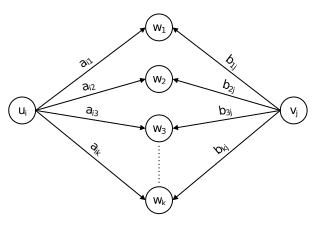
\includegraphics{layeredGraphInnerProduct.svg.png} 
  \caption[Rappresentazione grafica del calcolo di $c_{i,j}$ mediante Inner-product]
  \decoRule \label{fig:layeredGraphInnerProduct}
\end{figure}
Per la formulazione Inner-product \ref{fig:layeredGraphInnerProduct} 
è necessario esaminare ogni coppia di vertici  in U e V per trovare 
il sottoinsieme di $\tilde{W_{ij}} \subseteq W$ che connette coppie di nodi. \\
Vengono accumulati i prodotti $a_{il} \cdot b_{lj}$ relativi a $\tilde{W_{ij}}$ in $c_{ij}$.\\
È possibile osservare come la sparsità delle matrici non è sfruttata dato
che è necessario analizzare tutte le coppie di nodi $(u_i,v_j)$\\
%%OUTER PRODUCT
\begin{figure}[h]
  \centering 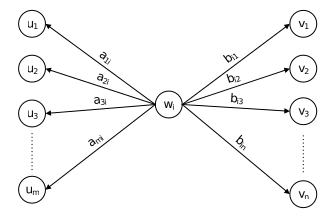
\includegraphics{layeredGraphOuterProduct.svg.png} 
  \caption[Rappresentazione grafica della componente $a_{*i} \cdot b_{i*}$ del calcolo di C mediante Outer-product]
  \decoRule \label{fig:layeredGraphOuterProduct}
\end{figure}
Per la formulazione Outer-product \ref{fig:layeredGraphOuterProduct}
è possibile identificare le coppie di vertici connesse a
partire dai nodi di W che, per matrici sufficientemente sparse,
può essere un operazione più veloce rispetto all'Inner-product.\\
%TODO si complica l'accumulazione dei risultati intermedi
%%row-by-row
\begin{figure}[h]
  \centering 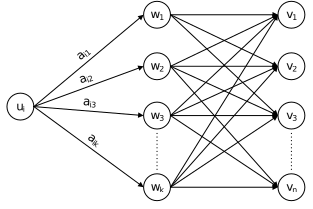
\includegraphics{layeredGraphRowByRow.svg.png} 
  \caption[Rappresentazione grafica della componente $a_{i*} \cdot B$ del 
     calcolo di C mediante formulazione row-by-row]
  \decoRule \label{fig:layeredGraphRowByRow}
  
\end{figure}
Per la formulazione Row-by-row \ref{fig:layeredGraphRowByRow}
le coppie di vertici d'interesse per il risultato di C sono identificabili 
a partire da attraversamenti del grafo indipendenti a partire dai vertici di U verso V.\\
%%col-by-col
Nel caso col-by-col vi è un attraversamento del grafo dai nodi di V a U, 
isomorfico rispetto al caso Row-by-row\\



\section{Algoritmi}
%%SRC STUDIES = Gustavson
Molte delle ricerche riguardo SpGEMM sono basate sull'algoritmo di Gustavson \parencite{gustavson},
un algoritmo sequenziale basato sulla formulazione Row-by-row, riportate in forma di pseudo-codice 
in \ref{figCode:gustavsonRigheSysSurvey} e graficamente in \ref{fig:gustavsonRigheGraphicalIntel}.\\

\begin{figure}[h]
  \caption[pseudo-codice dell'algoritmo di Gustavson]
  \centering 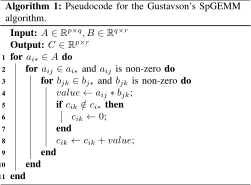
\includegraphics{gustavsonRigheSysSurvey.svg.png} \decoRule
  \label{figCode:gustavsonRigheSysSurvey}
\end{figure}
\begin{figure}[h]
  \caption[rappresentazione grafica di una iterazione dell'algoritmo di Gustavson]
  \centering 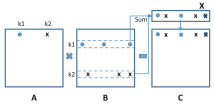
\includegraphics{gustavsonRigheGraphicalIntel.svg.png} \decoRule
  \label{fig:gustavsonRigheGraphicalIntel}
\end{figure}
È possibile notare come nell'algoritmo vi sia l'esigenza di accumulare le righe
risultanti della matrice C. Meccanismi efficienti per realizzare questa
funzionalità sono analizzati successivamente in \ref{ssec:gustavsonDerivate} %TODO FIX REF
\\


\section{Algoritmi paralleli multi-dimensionali} 
Gli algoritmi paralleli risolutivi del prodotto tra matrici possono essere
classificati in base al partizionamento del carico di lavoro sui processi.\\
\begin{figure}[h]
  \centering \includegraphics{pGEMM_cube.svg.png} 
  \caption[Rappresentazione grafica dell'assegnamento dei task per la risoluzione
      di SpGEMM in 1,2 e 3 dimensioni]\decoRule \label{fig:pGEMM_cube}
\end{figure}
%%WORKCUBE INTRO
L'assegnamento dei sotto problemi può essere visualizzato in un cubo di lavoro W \ref{fig:pGEMM_cube}
in cui ogni moltiplicazione di elementi \nnz $a_{i,k}*b_{k,j}$ è rappresentabile
con voxel $W(i,j,k)$ \parencite{cartesianPartitioningModels}.
Le proiezioni $W(i,j,k)$  sulle facce del cubo relative alle matrici A e B 
hanno elementi \nnz e determinano il pattern degl'elementi \nnz sulla matrice C.
%WORKCUBE NOTATIONS
\label{ch1:workCube}
I sottoinsiemi dei voxel di W ottenuti fissando uno o due indici sono denominati:
\begin{itemize}
  \item Layers: W(i,:,:),W(:,j,:),W(:,:,k)
  \item Fibers: Intersezioni di Layers relativi a indici diversi, e.g. W(i,j,:)
  \item Cuboid: Sottoinsiemi di W con tutte le dimensioni minori delle 
   dimensioni delle matrici corrispondenti
\end{itemize}

\subsection{Matrici ipersparse e rappresentazione DCSC}
È possibile definire una matrice sparsa A, come {\bf ipersparsa }se $nnz(A)$ è
inferiore alla sua dimensione più grande N \parencite{2dNewIdeas} \\ %TODO newIdeas 14.2.2 x matrici quadrate
Tipicamente questa tipologia di matrici è rara nell'algebra lineare numerica ma trova applicazioni
nel partizionamento di matrici sparse e nel processamento grafi, particolarmente se in parallelo.\\

Data una suddivisone bidimensionale di una matrice sparsa, %TODO quadrata
per un processamento parallelo in una griglia di p processi, si ha che ogni processo
verrà assegnato ad una matrice di dimensione circa $(n/\sqrt{p})~x~(n/\sqrt{p})$. %TODO ~~
L'occupazione globale di spazio di memoria sarà pari a 
$O(nnz + p \cdot n/\sqrt{p}) = O(nnz + n \cdot \sqrt{p})$ con CSC che è maggiore
dell'occupazione totale della matrice in un singolo processo $O(n + nnz)$.\\
Allo scalare del numero di processi p, il termine $n\sqrt{p}$ domina $nnz$.\\
%TODO The ineffciency of CSC leads to a more fundamental problem: any algorithm that
%uses CSC and scans all the columns is not scalable for hypersparse matrices. 
%Even without any communication at all, such an algorithm cannot scale for $n\sqrt{p} > \max{flops,nnz}$

Per queste ragioni è possibile utilizzare la rappresentazione 
{\bf D}ouble{\bf C}ompressed{\bf S}parse{\bf C}olumns,\ref{fig:DCSCvsCSC}
che ha un'occupazione di memoria pari ad $O(nnz)$
eliminando eventuali ripetizioni nell'array di puntatori delle colonne (JC) nel formato CSC.
È possibile favorire un rapido accesso alle colonne della matrice mediante un
array ausiliario di indici delle colonne \nnz
%TODO qualche spiegazione ulteriore
\begin{figure}[h]
  \caption[confronto delle rappresentazioni DCSC e CSC ]
  \centering 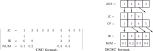
\includegraphics{DCSCvsCSC.svg.png} \label{fig:DCSCvsCSC}
\end{figure}

\subsection{Moltiplicazione tra matrici ipersparse rappresentate con DCSC}
\label{ssec:hypersparseGEMM}
Segue la descrizione di un algoritmo risolutivo per la moltiplicazione tra matrici
ipersparse \parencite{2dNewIdeas}, basato su una formulazione outer-product ed
utilizzato in alcuni algoritmi SpGEMM.\\
lo pseudo-codice dell'algoritmo è riportato in \ref{figCode:hypersparseGEMM} 


{\bf fase di preprocessamento} \\
viene effettuata una trasposizione di B, così da avere un indicizzamento rapido delle righe di B
in formato DCSC, necessario per la
formulazione outer-product.\\ 
%costo di trasposizione varia tra $O(n + nnz(B) \to nnz(B) lg nnz(b)) in base all implementazione
Viene effettuata l'intersezione tra gli indici delle colonne non zero di A e
delle righe non zero di B, identificando così il set $Isect = A.JC \cap B^T.JC$ degli
indici che partecipano all'outer-product.\\
\\
Successivamente vengono effettuati $|Isect|$ prodotti cartesiani \ref{fig:hypersparseGEMMGraphical} 
generanti matrici $a_{*i} \cdot b_{i*}$, i cui elementi è possibile mettere in biiezione 
con la lista di indici $(r_{id},c_{id})$ derivante dal prodotto cartesiano tra gli indici
di riga non zero della colonna i-esima di $B^T$ e gli indici di riga non zero 
della colonna i-esima di $A$.\\
La matrice risultante C può essere ottenuta mediante l'unione di queste liste,
sommando i contributi degl'elementi aventi gli stessi indici in liste
diverse.\\
Per implementare la costruzione di C dagli outer-products
è utilizzata una coda con priorità contenete elementi relativi ai
prodotti cartesiani per le colonne di $A$ e le colonne di $B^T ~\in~ Isect$, 
aventi per chiave $(r_{id},c_{id})$ e per valore il prodotto relativo e l'indice
della colonna di $A$ o $B^T$ relativa.\\
Verrà ripetutamente estratto il minimo dalla coda e reinserito
l'elemento successivo dalla lista di indici di relativa, sommando i
contributi di elementi con la stessa chiave.
I risultati verranno accumulati in uno stack mediante una rappresentazione
matriciale a coordinate degli elementi % TODO CHECK COO LIKE STACK ACCUMULATE
per poi essere convertiti nella matrice finale C in formato DCSC.\\

La complessità computazionale dell'algoritmo è $O(nzc(A) + nzr(B) +flops \cdot lg( ni))$
dove $ni$ è la dimensione della coda con priorità e $flops$ è il numero di
operazioni aritmetiche necessarie per il prodotto di A e B.\\

\begin{figure}[h]
  \centering 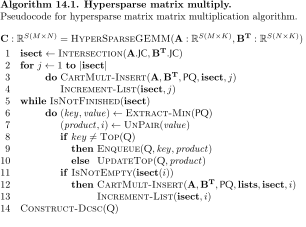
\includegraphics{hypersparseGEMM.svg.png}
  \caption[Algoritmo sequenziale per SpGEMM tra matrici ipersparse] \decoRule \label{figCode:hypersparseGEMM}
\end{figure}

\begin{figure}[h]
  \centering 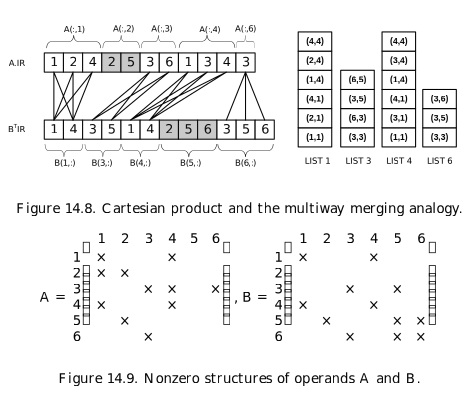
\includegraphics{hypersparseGEMMGraphical.svg.png}
  \caption[Rappresentazione grafica del prodotto cartesiano 
   a supporto di hypersparseGEMM ] \decoRule \label{fig:hypersparseGEMMGraphical}
\end{figure}


\subsection{Algoritmi con un partizionamento 2D}

\subsubsection{Derivati di Gustavson} \label{ssec:gustavsonDerivate}
Una parallelizzazione della formulazione per righe dell'algoritmo di Gustavson è
descritta in \parencite{intelSpGEMMDenseAccumulator}, sfruttando la
rappresentazione di matrici sparse in formato CSR.  \label{ssec:intelSpGEMMDenseAccumulator}
Lo pseudocodice dell'algoritmo è riportato in \ref{figCode:gustavsonRigheBlocksIntel}
e una sua rappresentazione grafica è raffigurata in
\ref{fig:gustavsonRigheBlocksGraphicalIntel}\\
%Partizionamento = Gustvason a blocchi
Viene effettuato un partizionamento delle righe di A e delle colonne di B e 
coppie di partizioni corrispondenti vengono utilizzate per calcolare un
blocco bidimensionale della matrice risultante C.\\
%accumulatore denso X
In accordo con la formulazione per righe dell'algoritmo di Gustavson, vengono
accumulati i contributi degli elementi \nnz delle righe di A e corrispettive porzioni
delle righe di B relative al calcolo di un blocco di C. 
Per effettuare efficientemente questa operazione, i vettori sparsi risultanti
dalle iterazioni dell'algoritmo, vengono accumulati in vettore denso X, 
semplicemente sommandone le componenti \nnz nelle relative locazioni di X.\\
%alternative memory efficient con overhead
In questa formulazione del problema, una soluzione di accumulazione 
alternativa potrebbe essere quella di accumulare i contributi per una riga di C 
utilizzando una hash-table di elementi aventi per chiave l'indice di colonna. 
Tuttavia, quest'approccio ha lo svantaggio di avere l'overhead relativo alla 
computazione delle funzioni hash e gestione di eventuali liste di collisione.\\
%implementazione conversione
Al termine del calcolo di una riga di un blocco di C, l'accumulare X viene
convertito in una riga CSR con l'ausilio di un ulteriore vettore di indici di
elementi \nnz sommati in X.\\
%Nota su partizionamento -> MENO cache miss su X
Utilizzando un partizionamento delle colonne di B è possibile partizionare anche
l'accumulatore X relativo ad una riga risultante di C. In questa maniera si
riduce il numero di cache line toccate dagli aggiornamenti di X, riducendo il
numero di cache miss relativi al ciclo interno dell'algoritmo.\\
Gli autori dell'algoritmo hanno verificato la riduzione di cache miss
utilizzando degli hardware counter per verificare il numero di cache miss L2
(tipicamente catturati dalla cache LLC) al variare del partizionamento di B % TODO QUANTIFICAZIONE?
%%Valutazione sul partizionamento di B -> X
%svantaggi
Tuttavia il partizionamento di B in rappresentazioni CSR separate, 
oltre che comportare un overhead computazionale, può comportare svantaggi in
termini di banda di memoria durante la lettura dei blocchi di B, che possono
essere notevolmente più sparsi della matrice originaria. %TODO link a ipersparse
%quantificazione euristica beneficio
Un beneficio dal partizionamento di B e di X, contro gli overhead citati, è
presente quando si ha certezza che per una significativa porzione delle righe
risultanti di C, l'occupazione dei \nnz, corrispondenti agli aggiornamenti
dell'accumulatore X, è maggiore della dimensione della cache L2.\\
Per quantificare il numero di \nnz nelle righe risultanti di C viene utilizzata
una metrica basata sulla stima di \nnz in $c_{i*}=e\_nnz(i)$ di
\parencite{intelSpGEMMDenseAccumulator} %TODO SOURCE ARTICLE OF ESTIMATE
dove si partiziona B se
$e\_nnz = \frac{\sum\limits_{i:e\_nnz(i) > L2\_FP\_WORDS} e\_nnz(i)}
{\sum\limits_{i=1}^m e\_nnz(i)} ~>~0.3$\\
%TODO scheduling dinamico -> load balancing con perizioni piccole t.c. #partizioni = 6-10 X #threads
\begin{figure}[h]
  \centering \includegraphics{gustavsonRigheBlocksIntel.svg.png}
  \caption[adattamento parallelo dell'algoritmo di Gustavson] \decoRule \label{figCode:gustavsonRigheBlocksIntel}
\end{figure}
\begin{figure}[h]
  \caption[rappresentazione grafica dell'adattamento parallelo dell'algoritmo di Gustavson] 
  \centering \includegraphics{gustavsonRigheBlocksGraphicalIntel.svg.png} \label{fig:gustavsonRigheBlocksGraphicalIntel}
\end{figure}

\subsubsection{Dense SUMMA} %versione base C=AB
Un partizionamento bidimensionale della risoluzione del prodotto tra matrici
dense è realizzato dell'algoritmo parallelo SUMMA \parencite{denseSumma} che è alla
base di una sua controparte per matrici sparse \parencite{sparseSUMMA}.\\
Il calcolo di $C=AB$ è suddiviso in sottomatrici assegnate a processi organizzati 
in una griglia bidimensionale di dimensione  $p_r x p_c$.\\
È possibile calcolare un blocco della matrice C come:
$C_{ij} =  \overbrace{\left(  A_{i1} | \dots |  A_{ip_c} \right)}^{\tilde{A^{i*}} }
~\cdot~ \overbrace{\left( 
        \begin{array}{c} B_{1j} \\ \vdots \\  B_{p_r j}
        \end{array} \right)} ^{\tilde{B^{*j}}} $\\
dove si usa la notazione:
\begin{itemize}
  \item $\tilde{a_{*l}}^{i*} \in \tilde{ A^{i*}}$ rappresenta 
    la colonna l-esima nella riga i-esima nella decomposizione a blocchi di A
  \item $\tilde{b_{l*}}^{*j} \in  \tilde{B^{*j}}$ rappresenta 
    la riga l-esima nella colonna j-esima nella decomposizione a blocchi di B.
\end{itemize}  
Applicando la formulazione outer-product su $\tilde{ A^{i*}}$ e $\tilde{B^{*j}}$
si ha che $C_{ij}=\sum\limits_{l=1}^{k}\tilde{a_{*l}}^{i*} \cdot \tilde{b_{l*}}^{*j}$\\
Considerando un partizionamento delle matrici in sottomatrici all'interno della
griglia di processi %assegnate in maniera tale che  ... 
si può eseguire l'operazione GEMM in parallelo come riportato dallo pseudocodice
in \ref{figCode:denseSUMMA}\\
\begin{figure}[h]
  \centering 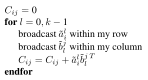
\includegraphics{denseSUMMA.svg.png}
  \caption[esecuzione dense SUMMA sul processo $P_{ij}$] \decoRule \label{figCode:denseSUMMA}
\end{figure}
Nell'articolo originale vengono discussi miglioramenti a questa formulazione
basati su uno scambio di dati tra i processi in un sistema a memoria distribuita
mediante una comunicazione ad anello 
riformulazione del calcolo di $C_{ij}$ utilizzando blocchi di
colonne di $\tilde{ A^{i*}}$ e righe di $\tilde{B^{*j}}$.\\

\subsubsection{Sparse SUMMA}
Un partizionamento bidimensionale del problema SpGEMM è realizzato
dall'algoritmo Sparse SUMMA \parencite{sparseSUMMA}, derivato dalla sua
controparte per matrici dense.\\
%SPARSE SUMMA
È riportato lo pseudo-codice dell'algoritmo sparseSUMMA 
in \ref{figCode:sparseSUMMA} e una sua iterazione graficamente in
\ref{fig:sparseSUMMAIteration}.\\
Le matrici sono divise in blocchi e rappresentante in formato DCSC,
trasponendo la matrice B per avere un indicizzamento rapido delle sue righe.\\
Procedendo in blocchi di colonne di una sottomatrice di A e della corrispettiva
sottomatrice di $B^T$, lungo la dimensione comune di A e B,
vengono calcolati in parallelo le sottomatrici $C_{ij}$, 
utilizzando l'algoritmo hypersparseGEMM \ref{ssec:hypersparseGEMM}.\\
Il costo computazionale dell'algoritmo è 
$O(\frac{dn}{\sqrt{p}}+\frac{d^2n}{p}lg(\frac{d^2n}{p}))$
%TODO CONSIDERAZIONE SU EFFICIENZA ALLO SCALARE DI p ... cmq no speedup bounds!
\begin{figure}[h]
  \caption[SparseSUMMA, per una risoluzione parallela di SpGEMM con un partizionamento 2D]
  \centering \includegraphics{sparseSUMMA.svg.png} \decoRule \label{figCode:sparseSUMMA}
\end{figure}
\begin{figure}[h]
  \caption[esecuzione di un iterazione dell'algoritmo sparseSUMMA]
  \centering \includegraphics{sparseSUMMAIteration.svg.png} \decoRule \label{fig:sparseSUMMAIteration}
\end{figure}

\subsection{Algoritmi con un partizionamento 3D}
Un partizionamento tridimensionale del problema SpGEMM è realizzato dall'
algoritmo Split-3D-SpGEMM \parencite{Split3DSpGEMM}, dove al partizionamento
bidimensionale descritto precedentemente, viene aggiunto una ulteriore
suddivisione delle sottomatrici in blocchi nella terza dimensione della griglia di processi.
%TODO CONSIDERAZIONI su overhead mem per C -> sparsity-structure dependent ->
%sfruttabile bene la sparsità del risultato in meno occupazione di memoria
Il partizionamento delle matrici è rappresentabile sul cubo di lavoro W come
riportato in figura \ref{fig:workCube3D}, dove il processo P(i,j,k) possiede la
porzione della matrice di A: 
$A(im/p_r:(i+1)m/p_r - 1, jn/p_c + kn/(p_c p_l ) : jn/p_c + (k + 1)n/(p_c p_l) - 1)$  \\
\begin{figure}[h]
  \caption[rappresentazione 3D della suddivisione della computazione SpGEMM]
  \centering \includegraphics{workCube3D.svg.png} \decoRule \label{fig:workCube3D}
\end{figure}
L'algoritmo è riportato nello pseudo-codice \ref{figCode:Split3DSpGEMM} e una
sua iterazione è raffigurata graficamente in \ref{fig:Split3DSpGEMMIteration}.\\

In maniera simile al caso di sparseSUMMA %TODO \ref{sparseSummaDescriptionStart}
si procede in parallelo calcolando il prodotto di sottoblocchi corrispondenti
alle sottomatrici di A e B, accumulando risultati intermedi la cui collocazione
è relativa all'intera fiber W(i,j,:).
Infine i risultati intermedi dei processi P(i,j,:), vengono distribuiti lungo la fiber
W(i,j,:), sommando i contributi relativi agli stessi indici.
\begin{figure}[h] 
  \caption[Split3DSpGEMM, per una risoluzione parallela di SpGEMM con un partizionamento 3D
     nel caso semplificato di una griglia di processi $\sqrt{p/c}~x~\sqrt{p/c}~x~c$]
  \centering 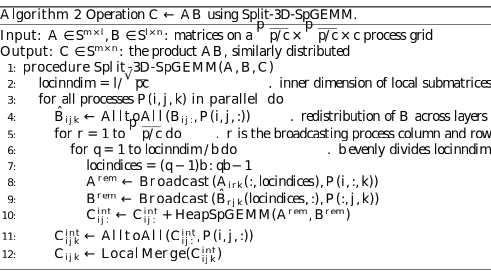
\includegraphics[width=1.0\textwidth]{Split3DSpGEMM.svg.png} \decoRule \label{figCode:Split3DSpGEMM}
\end{figure}
\begin{figure}[h]
  \caption[esecuzione di un iterazione dell'algoritmo Split3DSpGEMM]
  \centering \includegraphics[width=1.0\textwidth]{Split3DSpGEMMIteration.svg.png} 
  \decoRule \label{fig:Split3DSpGEMMIteration}
\end{figure}














%%Figure options
%%h 	Place the float here, i.e., approximately at the same point it occurs in the source text (however, not exactly at the spot)
%%t 	Position at the top of the page.
%%b 	Position at the bottom of the page.
%%p 	Put on a special page for floats only.
%%! 	Override internal parameters LaTeX uses for determining "good" float positions.
%%H 	Places the float at precisely the location in the LaTeX code. Requires the float package, though may cause problems occasionally. This is somewhat equivalent to h!.

\chapter{Implementazione OpenMp}
\label{Chapter2} % 2 reference \ref{Chapter2} 
%----------------------------------------------------------------------------------------

% Define some commands to keep the formatting separated from the content 
Prendendo spunto dalle caratteristiche principali degli algoritmi descritti
nella sezione precedente \ref{Chapter1}, 
ho realizzato alcune implementazioni per il prodotto tra matrici sparse con OpenMP,
considerando la formulazione row-by-row in \ref{Ch1:formulazioni} 
ed un partizionamento dei dati monodimensionale e bidimensionale.\\ 

\section{Determinazione della dimensione matrice risultante} \label{ch2:outSizeUB}
La dimensione della matrice risultante può essere determinata sia con un
UpperBound sia con in una modalità accurata con maggiore costo computazionale.\\
Ho scelto di adottare una soluzione efficiente per calcolare un UpperBound per la
dimensione della matrice risultante come riportato nell'algoritmo 4 di \parencite{sysReviewChi}.\\
In questa soluzione, ispirandosi a una formulazione row-by-row di SpGWMM, 
si determina la dimensione massima di ogni riga della matrice risultante come:\\
$ | I_i(C) |~\leq~\sum\limits_{ j \in I_i(A) }  | I_j(B) | $ 

\section{Accumulatore denso per i prodotti intermedi} %TODO descrizione generica oltre della sola form. row-by-row
Come analizzato da \parencite{intelSpGEMMDenseAccumulator}, precedentemente in 
\ref{ssec:intelSpGEMMDenseAccumulator} possono esserci diversi vantaggi 
nell'utilizzo di un accumulatore denso per i prodotti intermedi effettuati in SpGEMM.
%THREAD_AUX_VECT
Per questa ragione ho deciso di utilizzare questo stratagemma nella
computazione delle partizioni delle righe della matrice risultante in una
struttura di questo tipo:
\begin{lstlisting}
double* v;          //dense accumulator for intermediate products
uint*   nnzIdx;     //nonzero accumulated values indexes of v
uint    nnzIdxLast; //index of last appended non zero value in nnzIdx
\end{lstlisting}    %TODO uint    vLen;       
nella quale in \verb|v| vengono accumulati i prodotti intermedi 
ed in \verb|nnzIdx| vengono inseriti gli indici delle componenti non zero accumulate in \verb|v|.
%Dense acc size
Entrambi questi array devono essere allocati con uno spazio sufficiente a contenere
tutti i risultati dei prodotti intermedi da effettuare in un'iterazione di SpGEMM. \\
Nel caso della formulazione row-by-row 
\verb|v| rappresenterà gli elementi \nnz di una partizione di una riga della matrice risultate e
\verb|nnzIdx| rappresenteranno gli indici relativi, \emph{shiftati} di uno %TODO traslati..
spiazzamento da aggiungere, relativo a quale partizione della matrice risultate si sta calcolando.
È possibile sovrallocare questi vettori con il numero di colonne di una partizione della matrice B\\
%nnzIdx append 
Gl'indici dei valori non zero accumulati in \verb|v| sono inseriti consecutivamente grazie   
alla variabile \verb|nnzIdxLast|,contente l'indice dell'ultimo elemento inserito in \verb|nnzIdx|
il quale corrisponde ad un buon UpperBound del numero di valori non zero accumulati .\\

\subsection{Trasformazione da un accumulatore denso in un vettore sparso}  %sparsifyDenseVect
\label{ch2:sparsifyDenseVect}
È necessario trasformare l'accumulatore denso appena descritto in un 
formato sparso per ottenere la matrice risultate, copiando gli elementi \nnz 
in \verb|v| e i relativi indici nella struttura sparsa di destinazione.\\
%Esigenza vettore sparso come step intermedio
Data la generazione parallela degli accumulatori densi
ho scelto di utilizzare dei vettori sparsi ausiliari, rappresentanti porzioni della matrice risultate, 
piuttosto che scrivere gli elementi \nnz di \verb|v| direttamente nell' output di SpGEMM,
%alternativa senza accSparso intermedio con troppa sincronizzazione / predizione & memove & realloc
data la difficile determinazione dell'offset al quale copiare gli elementi \nnz e la relativa sincronizzazione necessaria.

\subsubsection{Allocazione vettori sparsi intermedi}
La dimensione dei vettori sparsi intermedi, generati in parallelo,
non è nota prima di ottenere gli accumulatori densi a meno di non effettuare 
una precomputazione simbolica dell'intera operazione SpGEMM come indicato in \parencite{sysReviewChi}.\\
Nell'ipotesi di usare una parallelizzazione di SpGEMM sfruttando la direttiva OpenMp,
\begin{lstlisting}[numbers=none]
#pragma omp parallel for 
\end{lstlisting} %TODO ANCHE A LIVELLO GENERALE in costrutti work-sharing? 
effettuare delle operazioni che potrebbero causare errori, come delle malloc,
e quindi la terminazione  anticipata del ciclo parallelizzato, 
vanno contro la filosofia OpenMP secondo cui il numero di iterazioni del ciclo
da parallelizzare deve essere precomputabile prima del ciclo stesso. \\ 
%TODO KEEP? omp cancel disabled by dflt
%A sostegno della filosifa OpenMP riguardo la precomputabilità del numero di iterazioni di un ciclo parallelizzato 
A sostegno di ciò c'è che il costrutto che potrebbe consentire una uscita anticipata dal ciclo:
\begin{lstlisting}[numbers=none]
#pragma omp cancel for 
\end{lstlisting} 
è disabilitato a meno di essere abilitato esplicitamente mediante la 
Internal Control Variable \verb|cancel-var | \parencite{openmp5.1}\\
     % TODO DOUBLE CHECK: per motivi di performance

Per questo motivo, ho deciso di effettuare una preallocazione di uno spazio
sufficiente a contenere tutti gli elementi \nnz della matrice risultante, come
descritto in \ref{ch2:outSizeUB} per poi assegnarne porzioni ai vari thread 
che necessitano di \emph{sparsificare} un accumulatore denso in un accumulatore 
sparso mediante una primitiva atomica di sincronizzazione.\\

Una semplificazione della trasformazione dell'accumulatore denso in un
accumulatore sparso è riportata nel blocco di codice seguente
%%static inline void sparsifyDenseVect
\begin{lstlisting}
uint nnz = accDenseV -> nnzIdxLast, accSparseStartIdx;
sortuint(accDenseV->nnzIdx,nnz); //sort nnz idx for ordered write
accSparse -> len = nnz;
//sparse accumulator space atomic assign
accSparseStartIdx = __atomic_fetch_add(&(accDense->lastAssigned),nnz,__ATOMIC_SEQ_CST); 
accSparse -> AS = accDense->AS + accSparseStartIdx; 
accSparse -> JA = accDense->JA + accSparseStartIdx; 
///sparsify dense acc.v into row
for (uint i=0,j;    i<nnz;   i++){ 
    j = accDenseV -> nnzIdx[i]; //shifted 
    accSparse -> JA[i] = j + startColAcc;
    accSparse -> AS[i] = accDenseV->v[j];
}
\end{lstlisting}
in cui si riserva uno spazio per il nuovo accumulatore sparso \verb|accSparse|
nelle righe 5-7.\\
In particolare ho utilizzato un contatore per gli elementi già assegnati dalla
preallocazione iniziale il cui accesso è gestito dalla primitiva di sincronizzazione 
\verb|__atomic_fetch_add| in riga 5, per ottenere il suo valore corrente 
ed incrementarlo atomicamente del numero di elementi \nnz dell'accumulatore denso 
%così da simulare una allocazione 
.\\
%sort nnzIdx array
Gli indici degli elementi \nnz inseriti in \verb|nnzIdx| è relativo all'ordine
degli elementi \nnz incontrati durante i prodotti intermedi e necessita quindi
di un riordinamento, fatto a riga 2 
sfruttando la funzione \verb|qsort| inclusa nella \verb|glibc|.
Il riordinamento non ha un grande impatto sulle performance dato che 
è effettuato in parallelo su ogni partizione della matrice risultante che,
essendo sparse, contengono potenzialmente pochi elementi \nnz .\\
%NOTA SU QUICK SORT OTTIMIZZATO https://elixir.bootlin.com/glibc/glibc-2.34.9000/source/stdlib/qsort.c#L89
Infine effettuo la copia dei soli valori \nnz nelle righe 10-12,
%shift back from scSparseVectMulPart 
avendo cura di trasformare gli indici degli elementi \nnz da relativi al solo
accumulatore ad assoluti rispetto alla matrice risultante

%TODO EVENTUALMENTE ? PARTE RELATIVA TRIPLO PRODOTTO DIRETTO VS  COPPIA DI SPGEMM

\section{Partizionamento monodimensionale}
Un semplice partizionamento delle matrici per parallelizzare l'operazione di
moltiplicazione tra matrici sparse $A * B$ in una formulazione row-by-row è quello di 
assegnare righe o blocchi di righe della matrice A ai thread.
Nella terminologia introdotta precedentemente in \ref{ch1:workCube}, equivale ad
assegnare gruppi di Layers del cubo di lavoro ai vari threads.\\
Segue una parte del codice per effettuare l'operazione di SpGEMM con 
un partizionamento per blocchi di righe della matrice A:    \label{ch2:part1DGroup}
\begin{lstlisting}
    #pragma omp parallel for schedule(runtime) private(acc,startRow,block)
    for (b=0;   b < conf->gridRows; b++){
        block     = UNIF_REMINDER_DISTRI(b,rowBlock,rowBlockRem);
        startRow  = UNIF_REMINDER_DISTRI_STARTIDX(b,rowBlock,rowBlockRem);
        //row-by-row formulation in the given row block
        for (uint r=startRow;  r<startRow+block;  r++){
            //iterate over nz entry index c inside current row r
            accDense = accVects + b;
            for (uint c=A->IRP[r]; c<A->IRP[r+1]; c++) 
                scSparseRowMul(A->AS[c], B, A->JA[c], accDense );
            //trasform accumulated dense vector to a CSR row
            sparsifyDenseVect(outAccumul,acc,outAccumul->accs + r,0);
            _resetAccVect(accDense);   //rezero for the next A row
        }
    }
    ///merge sparse row computed before
    if (mergeRows(outAccumul->accs,AB))    goto _err;
\end{lstlisting}
Data una rappresentazione CSR delle matrici, è possibile effettuare un 
partizionamento delle righe semplicemente suddividendo gli indici degli elementi
\nnz tramite il vettore degli offset iniziali delle righe \verb|IRP|,
come fatto nelle righe 2-6.\\
La i-esima riga di C è calcolata come 
$c_{i*} = \sum\limits_{k \in I_i(A)}  a_{ik} \ast  b_{k*}$  in un accumulatore denso
nelle righe 9-10.\\
Successivamente gli accumulatori densi vengono convertiti in accumulatori sparsi
in \verb|sparsifyDenseVect| come precedentemente descritto \ref{ch2:sparsifyDenseVect}
per poi essere copiati nella matrice risultante in \verb|mergeRows| a riga 17.

\section{Partizionamento bidimensionale}
Un partizionamento 2D delle matrici in input è quello di assegnare ai threads 
blocchi bidimensionali della matrice C ottenuti dalla moltiplicazione di
blocchi di righe della matrice A e blocchi di colonne della matrice B.\\
Nella terminologia introdotta precedentemente in \ref{ch1:workCube}, equivale ad
assegnare gruppi di fibers del cubo di lavoro ai vari threads.\\

\subsection{Partizionamento colonne di una matrice CSR mediante offset}
Per partizionare le colonne di una matrice CSR è possibile utilizzare una
matrice di indici di supporto contenete per ogni riga l'indice iniziale di ogni
partizione. Segue la funzione per effettuare questo partizionamento:
\begin{lstlisting}
/*
 * partition CSR sparse matrix @A in @gridCols columns partitions 
 * returning an offsets matrix out[i][j] = start of jth colPartition of row i
 * subdivide @A columns in uniform cols ranges in the output 
 */
uint* colsOffsetsPartitioningUnifRanges(spmat* A,uint gridCols){
    uint subRowsN = A->M * gridCols;
    uint _colBlock = A->N/gridCols, _colBlockRem = A->N%gridCols;
    uint* offsets = malloc( (subRowsN+1) * sizeof(*offsets) );
    if (!offsets)  {
        ERRPRINT("colsOffsetsPartitioning:\t offsets malloc errd\n");
        return NULL;
    }
    ///OFFSETS COMPUTE FOR COL GROUPS -> O( A.NZ )
    for (uint r=0, j=0;     r<A->M;     j=A->IRP[++r]){
        //navigate column groups inside current row
        for (uint gc=0,gcStartCol=0;  gc<gridCols;  gc++){
            //goto GroupCols start entry keeping A's nnz entries navigation (j)
            while ( j < A->IRP[r+1] &&  A->JA[j] < gcStartCol )  j++;
            offsets[ IDX2D(r,gc,gridCols) ] = j;//row's part start
            gcStartCol += UNIF_REMINDER_DISTRI(gc,_colBlock,_colBlockRem);
        }
    }
    offsets[subRowsN] = A->NZ;
    return offsets;
}
\end{lstlisting}
Per calcolare l'indice iniziale delle partizioni per ogni riga si valutano gli
elementi \nnz della matrice fino ad averne uno con indice di colonna $\geq$
dell'indice iniziale della partizione a riga 19

\subsection{Partizionamento colonne di una matrice CSR in matrici separate}
Un partizionamento per colonne alternativo di una matrice CSR consiste in una
allocazione di matrici CSR dedicate per ogni partizione con una sovrallocazione
inziale degli elementi \nnz.\\
Segue il principale blocco di codice per effettuare questo partizionamento:

\begin{lstlisting}
//for each A cols part -> last copied nz index = nnz copied ammount
uint* colPartsLens = alloca(gridCols * sizeof(colPartsLens));
memset(colPartsLens, 0, sizeof(*colPartsLens) * gridCols);
//OFFSET BASED COPY OF A.COL_GROUPS -> O( A.NZ )
for (uint r=0, j=0;     r<A->M;     j=A->IRP[++r]){
    //navigate column groups inside current row
    for (uint gc=0,gcEndCol=0,i;  gc<gridCols ;  gc++,j+=i){
        i = 0;  //@i=len current subpartition of row @r to copy
        colPart = colParts + gc;
        colPart->IRP[r] = colPartsLens[gc];
        gcEndCol += UNIF_REMINDER_DISTRI(gc,_colBlock,_colBlockRem);
        //goto next GroupCols,keeping A's nnz entries navigation (j+i)
        while ( j+i < A->IRP[r+1] && A->JA[j+i] < gcEndCol ) i++;
        memcpy(colPart->AS+colPart->IRP[r],A->AS+j,i*sizeof(*(A->AS)));
        memcpy(colPart->JA+colPart->IRP[r],A->JA+j,i*sizeof(*(A->JA)));
        
        colPartsLens[gc] += i;
    }
}
\end{lstlisting}

Tenendo traccia del numero di elementi \nnz copiati per ogni partizione nel
vettore \verb|colPartsLens| è possibile aggiornare l'indice iniziale di riga 
delle partizioni a riga 10 ed a riga 14, in maniera simile al partizionamento
precedente, si identifica il confine della partizione corrente per poi
effettuare la copia dei valori \nnz della partizione nelle righe 14,15.\\ %TODO meno ripetizioni ?

Considerando quest'ultimo tipo di partizionamento delle colonne della matrice B 
ed utilizzando il partizionamento precedente per gruppi di righe della matrice A
\ref{ch2:part1DGroup}, l'operazione di SpGEMM è effettuata mediante il codice seguente:
\begin{lstlisting}
#pragma omp parallel for schedule(runtime) private(accV,accRowPart,\
  colPart,rowBlock,colBlock,startRow,startCol,t_i,t_j)
for (tileID = 0; tileID < gridSize; tileID++){
    ///get iteration's indexing variables
    //tile index in the 2D grid of AB computation 
    t_i = tileID/conf->gridCols;  //i-th row block
    t_j = tileID%conf->gridCols;  //j-th col block
    //get tile row-cols group FAIR sizes
    rowBlock = UNIF_REMINDER_DISTRI(t_i,_rowBlock,_rowBlockRem); 
    colBlock = UNIF_REMINDER_DISTRI(t_j,_colBlock,_colBlockRem);
    startRow = UNIF_REMINDER_DISTRI_STARTIDX(t_i,_rowBlock,_rowBlockRem);
    startCol = UNIF_REMINDER_DISTRI_STARTIDX(t_j,_colBlock,_colBlockRem);
    
    colPart = colPartsB + t_j;
    accV = accVectors + tileID; 
     
    ///AB[t_i][t_j] block compute
    for (uint r=startRow;  r<startRow+rowBlock;  r++){
        //iterate over nz col index j inside current row r
        //row-by-row restricted to colsubset of B to get AB[r][:colBlock:]
        for (uint j=A->IRP[r],c,bRowStart,bRowLen; j<A->IRP[r+1]; j++){
            //get start of B[A->JA[j]][:colBlock:]
            c = A->JA[j]; // column of nnz entry in A[r][:] <-> target B row
            bRowStart = colPart->IRP[c];
            bRowLen   = colPart->IRP[c+1] - bRowStart;
            scSparseVectMulPart(A->AS[j],colPart->AS+bRowStart,
                colPart->JA+bRowStart, bRowLen,startCol,accV);
        }

        accRowPart = outAccumul->accs + IDX2D(r,t_j,conf->gridCols);
        sparsifyDenseVect(outAccumul,accV,accRowPart,startCol);
        _resetAccVect(accV);
    }
}
    if (mergeRowsPartitions(outAccumul->accs,AB,conf))  goto _err;
\end{lstlisting}
Ogni thread è associato a un blocco da calcolare bidimensionale della matrice C
identificato dagl'indici \verb|t_i| \verb|t_j| a riga 6 e 7,
moltiplicando un blocco di righe della matrice A e un blocco di colonne della matrice
B identificati dalle variabili in rige 9-12.\\
Nel ciclo a riga 21, ogni thread computerà la porzione della riga \verb|r| di C
relativa alla dimensione della partizione corrente di B a lui associata in un
accumulatore denso.
Successivamente ogni thread provvederà a trasformare l'accumulatore denso in uno
sparso mediante \verb|sparsifyDenseVect|, tenendo conto della colonna della
sua partizione.\\
Infine, mediante \verb|mergeRowsPartitions| i vari vettori sparsi accumulati
in una struttura di supporto dai thread, verranno uniti nella matrice risultante.\\
 

%%----------------------------------------------------------------------------------------
%%	THESIS CONTENT - APPENDICES
%%----------------------------------------------------------------------------------------
%
%\appendix % Cue to tell LaTeX that the following "chapters" are Appendices
%
%% Include the appendices of the thesis as separate files from the Appendices folder
%% Uncomment the lines as you write the Appendices
%
%% Appendix A

\chapter{Frequently Asked Questions} % Main appendix title

\label{AppendixA} % For referencing this appendix elsewhere, use \ref{AppendixA}

\section{How do I change the colors of links?}

The color of links can be changed to your liking using:

{\small\verb!\hypersetup{urlcolor=red}!}, or

{\small\verb!\hypersetup{citecolor=green}!}, or

{\small\verb!\hypersetup{allcolor=blue}!}.

\noindent If you want to completely hide the links, you can use:

{\small\verb!\hypersetup{allcolors=.}!}, or even better: 

{\small\verb!\hypersetup{hidelinks}!}.

\noindent If you want to have obvious links in the PDF but not the printed text, use:

{\small\verb!\hypersetup{colorlinks=false}!}.

%%\include{Appendices/AppendixB}
%%\include{Appendices/AppendixC}
%
%%----------------------------------------------------------------------------------------
%%	BIBLIOGRAPHY
%%----------------------------------------------------------------------------------------
%
\printbibliography[heading=bibintoc]

%----------------------------------------------------------------------------------------

\end{document}  
